

\id{МРНТИ 06.71.57}

{\bfseries ҚАЗАҚСТАННЫҢ ТУРИСТІК СЕКТОРЫНДАҒЫ КӘСІПКЕРЛІК БЕЛСЕНДІЛІКТІ
ҚОЛДАУ}

{\bfseries \textsuperscript{1}А.Сабыржан\textsuperscript{\envelope },
\textsuperscript{2}Г.К.Абдраманова},
{\bfseries \textsuperscript{2}А.Т.Тлеубаева},
{\bfseries \textsuperscript{2}М.С.Сиеубаева}

\textsuperscript{1} Е.А.Бөкетов атындағы Қарағанды университеті,
Қарағанды, Қазақстан,

\textsuperscript{2}Л.Н. Гумилев атындағы Еуразия ұлттық университеті,
Астана, Қазақстан

{\bfseries \textsuperscript{\envelope }}Корреспондент-автор:
Alisher-aliev-79@mail.ru

Бұл мақала Қазақстан Республикасындағы туристік кәсіпкерлікті дамытудағы
технологиялар мен инновациялардың рөлін талдауға арналған.
Егжей-тегжейлі статистикалық талдау негізінде авторлар туризм
индустриясының өсу динамикасына әсер ететін негізгі макроэкономикалық
жағдайлар мен факторларды анықтайды. Жұмыста ұзақ мерзімді экономикалық
дамуды қамтамасыз ету үшін экономиканы әртараптандырудың және туристік
сектордың тұрақтылығының маңыздылығы көрсетілген. 2022 жылы туристер
санының 9 миллионнан астам өскенін көрсететін статистикалық деректерді
талдау келтірілген, бұл өткен жылдың көрсеткіштерінен 20\% - ға жоғары.
2021 жылы 88,9 млрд теңгені құраған, ал 2023 жылдың басында 98,7 млрд
теңгеге жеткен туристік қызметтен түсетін табыс көрсеткіштері қаралды.

Зерттеу туристік қызметтердің сапасын жақсарту және бәсекеге
қабілеттілікті арттыру үшін цифрлық технологияларды енгізу сияқты
инновациялық тәсілдердің маңыздылығын көрсетеді. Сапалы қонақ үйлердің
тапшылығын және экскурсиялық инфрақұрылымның жеткіліксіз дамуын қоса
алғанда, инфрақұрылымдық шектеулердің туристік ағынның өсуіне әсері
қарастырылуда. Жою үшін туристік инфрақұрылымды жаңғыртуға және
кеңейтуге стратегиялық инвестициялар ұсынылды.

Мақалада ұлттық саябақтар сияқты 200-ден астам қорғалатын табиғи
аумақтарды пайдалануды қоса алғанда, экологиялық және мәдени туризмнің
әлеуеті қарастырылады. Болжамдарға сүйене отырып, мемлекеттік қолдаудың,
кластерлік тәсілді дамытудың және халықаралық туристерді тарту үшін
маркетингтік стратегияларды қолданудың маңыздылығы атап өтіледі.

Ағымдағы трендтерді талдай отырып, авторлар нормативтік-құқықтық базаны
жетілдіру, кредиттеуді жеңілдету және ұлттық туристік өнімді ілгерілету
арқылы кәсіпкерлік белсенділікті одан әрі ынталандыру қажеттілігі туралы
қорытындыға келеді. Қонақүйлердің жүктемесін арттыру (70\%) және
халықаралық орналастыру объектілерінің санын 228 бірлікке ұлғайту туралы
деректерді пайдалана отырып, көрсеткіштер ағымдағы кедергілер жойылған
жағдайда туристік бизнестің өсу перспективаларын көрсетеді. Зерттеу
Қазақстанда туризмнің табысты дамуы экономикалық, әлеуметтік және
инфрақұрылымдық ресурстарды интеграциялауға бағытталған кешенді тәсілді
талап ететінін атап көрсетеді. Трендтік модельдерге негізделген
болжамдар саладағы оң үрдістерді растайды, бұл елдің экономикалық
дамуына айтарлықтай үлес қосатынын көрсетеді.

{\bfseries Түйін сөздер:} туристік сала, кәсіпкерлік субъектілері,
кәсіпкерлік белсенділік, даму факторлары, әртараптандыру, тұрақтылық,
туроператор, Инфрақұрылым.

{\bfseries ПОДДЕРЖКА ПРЕДПРИНИМАТЕЛЬСКОЙ АКТИВНОСТИ В ТУРИСТСКОМ СЕКТОРЕ
КАЗАХСТАНА}

{\bfseries \textsuperscript{1}А.Сабыржан\textsuperscript{\envelope },
\textsuperscript{2}Г.К.Абдраманова},
{\bfseries \textsuperscript{2}А.Т.Тлеубаева}, {\bfseries \textsuperscript{2}М.
С.Сиеубаева}

\textsuperscript{1} Карагандинский университет имени Е.А. Букетова,
Караганда, Казахстан,

\textsuperscript{2}Л.Н. Гумилев атындағы Еуразия ұлттық университеті,
Астана, Казахстан,

e-mail:
\href{mailto:Alisher-aliev-79@mail.ru}{\nolinkurl{Alisher-aliev-79@mail.ru}}

Данная статья посвящена анализу роли технологий и инноваций в развитии
туристического предпринимательства в Республике Казахстан. На основе
детального статистического анализа, авторы выявляют основные
макроэкономические условия и факторы, оказывающие влияние на динамику
роста туристической индустрии. В работе подчёркивается значение
диверсификации экономики и устойчивости туристического сектора для
обеспечения долгосрочного экономического развития. Приведён анализ
статистических данных, демонстрирующие увеличение числа туристов более 9
миллионов в 2022 году, что на 20\% выше показателей предыдущего года.
Рассмотрены показатели дохода от туристической деятельности, который в
2021 году составил 88,9 млрд тенге, а в начале 2023 года достиг 98,7
млрд тенге.

Исследование выделяет значимость инновационных подходов, таких как
внедрение цифровых технологий, для повышения качества туристических
услуг и увеличения конкурентоспособности. Рассматривается влияние
инфраструктурных ограничений, включая дефицит качественных гостиниц и
недостаточное развитие экскурсионной инфраструктуры, на рост
туристического потока. Для устранения предложены стратегические
инвестиции в модернизацию и расширение туристической инфраструктуры.

В статье рассматривается потенциал экологического и культурного туризма,
включая использование более 200 охраняемых природных территорий, таких
как национальные парки. Основываясь на прогнозах, подчёркивается
важность государственной поддержки, развития кластерного подхода и
использования маркетинговых стратегий для привлечения международных
туристов.

Анализируя текущие тренды, авторы приходят к выводу о необходимости
дальнейшего стимулирования предпринимательской активности через
совершенствование нормативно-правовой базы, облегчение кредитования и
продвижение национального турпродукта. Используя данные о повышении
загрузки гостиниц (70\%) и увеличении числа международных объектов
размещения, в количестве 228 единиц, показатели демонстрируют
перспективы роста туристического бизнеса при условии устранения текущих
барьеров.

Исследование подчёркивает, что успешное развитие туризма в Казахстане
требует комплексного подхода, направленного на интеграцию экономических,
социальных и инфраструктурных ресурсов. Прогнозы, основанные на
трендовых моделях, подтверждают положительные тенденции в отрасли, что
говорит о значительном вкладе в экономическое развитие страны.

{\bfseries Ключевые слова:} туристская сфера, субъекты предпринимательства,
предпринимательская активность, факторы развития, диверсификация,
стабильность, туроператор, инфраструктура{\bfseries .}

{\bfseries SUPPORT FOR ENTREPRENEURIAL ACTIVITY IN THE TOURISM SECTOR OF
KAZAKHSTAN}

{\bfseries \textsuperscript{1}A.Sabyrzhan\textsuperscript{\envelope },
\textsuperscript{2}G.Abdramanova , \textsuperscript{2}A.Tleubayeva ,
\textsuperscript{2}M.Siyeubayeva}

\textsuperscript{1} Karaganda Buketov University, Karaganda, Kazakhstan,

\textsuperscript{2}L.N. Gumilyov Eurasian National University, Astana,
Kazakhstan,

e-mail:
\href{mailto:Alisher-aliev-79@mail.ru}{\nolinkurl{Alisher-aliev-79@mail.ru}}

This article is devoted to the analysis of the role of technologies and
innovations in the development of tourism entrepreneurship in the
Republic of Kazakhstan. Based on a detailed statistical analysis, the
authors identify the main macroeconomic conditions and factors
influencing the growth dynamics of the tourism industry. The paper
emphasizes the importance of economic diversification and the
sustainability of the tourism sector to ensure long-term economic
development. The analysis of statistical data showing an increase in the
number of tourists of more than 9 million in 2022, which is 20\% higher
than the previous year.

The indicators of income from tourism activities, which in 2021 amounted
to 88.9 billion tenge, and in early 2023 reached 98.7 billion tenge, are
considered. The study highlights the importance of innovative
approaches, such as the introduction of digital technologies, to improve
the quality of tourism services and increase competitiveness. The impact
of infrastructural constraints, including a shortage of high-quality
hotels and insufficient development of excursion infrastructure, on the
growth of tourist flow is considered. Strategic investments in the
modernization and expansion of tourism infrastructure are proposed to
eliminate this problem. The article discusses the potential of
ecological and cultural tourism, including the use of more than 200
protected natural areas such as national parks.

Based on the forecasts, the importance of government support, the
development of a cluster approach and the use of marketing strategies to
attract international tourists is emphasized. Analyzing current trends,
the authors conclude that it is necessary to further stimulate
entrepreneurial activity through improving the regulatory framework,
facilitating lending and promoting national tourism products. Using data
on an increase in hotel occupancy (70\%) and an increase in the number
of international accommodation facilities, in the amount of 228, the
indicators demonstrate the prospects for the growth of the tourism
business, provided that current barriers are eliminated. The study
emphasizes that the successful development of tourism in Kazakhstan
requires an integrated approach aimed at integrating economic, social
and infrastructural resources. Forecasts based on trend models confirm
positive trends in the industry, which indicates a significant
contribution to the economic development of the country.

{\bfseries Keywords:} tourism industry, business entities, entrepreneurial
activity, development factors, diversification, sustainability, tour
operator, infrastructure.

{\bfseries Кіріспе.} Қазақстанның туристік индустриясы экономиканы
әртараптандыруға және орнықты дамуға ықпал ететін маңызды секторлардың
бірі болып табылады. 2022 жылы елдегі туристер саны 9 миллионнан асты,
бұл 2021 жылғы деңгейден 20\% жоғары. Туристік қызметтен түсетін табыс
2021 жылғы 88,9 млрд теңгеден 2023 жылы 98,7 млрд теңгеге дейін ұлғайды,
бұл саланың оң серпінін көрсетеді. Алайда, қазақстандық туризмнің
әлемдік туристік индустрияға қосқан үлесі шектеулі болып қалып отыр, бұл
жалпы ағынның 1\% - дан азын құрайды. Несиелендірудің қол жетімділігі,
жалақы деңгейі және туристік инфрақұрылымның сапасы сияқты
макроэкономикалық факторлар саланың дамуына айтарлықтай әсер етеді. 2023
жылдың басында Қазақстанда 2851 қонақ үй жұмыс істейді, оның ішінде
халықаралық деңгейдегі 228 нысан, орташа жүктемесі 70 \%.

Дегенмен, сапалы қонақ үй қызметтерінің тапшылығы және белсенді және
мәдени туризм үшін инфрақұрылымның жеткіліксіз дамуы байқалады.
Жаһандану жағдайында саланың бәсекеге қабілеттілігін арттыру үшін
инновациялар мен инфрақұрылымдық жобаларға стратегиялық инвестициялау
қажет. Цифрлық технологияларды пайдалану қызмет көрсету сапасын
жақсартуға және Қазақстанның халықаралық туристер үшін тартымдылығын
арттыруға ықпал етеді.

Мысалы, ұлттық саябақтарды қоса алғанда, 200-ден астам қорғалатын табиғи
аумақтар экологиялық туризмді дамыту үшін жоғары әлеуетке ие. Мақалада
"Қазақстанда туристік индустрияны дамыту инновациялық технологияларды
интеграциялау, инфрақұрылымды жақсарту және ресурстарды стратегиялық
басқару арқылы мүмкін болады, бұл саланың бәсекеге қабілеттілігін және
ел экономикасына қосқан үлесін арттыруға мүмкіндік береді"деген ғылыми
гипотеза қалыптастырылды. Зерттеу туризмді дамыту бағдарламаларын іске
асыруды және кластерлік тәсілді енгізуді қоса алғанда, мемлекеттік
ынталандырудың маңыздылығын көрсетеді. Трендтік модельдерге негізделген
2023-2025 жылдарға арналған болжамдар ағымдағы кедергілерді жою және
ресурстарды пайдалануды оңтайландыру шартымен саланың тұрақты өсуін
растайды. Мақалада ағымдағы проблемаларды еңсеруге және оның ел
экономикасына қосқан үлесін арттыру үшін саланың әлеуетін пайдалануға
бағытталған Қазақстандағы туристік кәсіпкерлікті дамытуға кешенді
көзқарас қажеттілігі негізделеді.

{\bfseries Материалдар мен әдістер.} Туризм экономикалық өсу мен қалпына
келтірудің маңызды қозғаушы күші болып табылады {[}1{]}. Туристік
ресурстармен қамтамасыз ету маңызды рөл атқарады, өйткені туристер мен
инвесторларды көбірек тарту үшін тартымды орындар мен нысандардың болуы
{[}2{]}.

Қаржы ресурстарын оңтайлы бөлу және білікті бағыт әлеуметтік ресурстарды
тиімдірек пайдалануға ықпал етеді, яғни туристік индустриядағы қаржыны
дұрыс басқару кірістердің өсуіне және туристік қызметтердің сапасын
жақсартуға ықпал етеді {[}3{]}. Туризм индустриясы Қазақстан
Республикасын дамытудың басым бағыттарының қатарына кіреді. Ұлттық
туризмді дамытуда отандық туристік кластерлер жүйесіне жетекші рөл
беріледі. Алайда, қазақстандық туризм әзірге ел экономикасына елеулі
үлес қоспай отыр, оның үлесіне әлемдік туристік ағынның 1\% - дан азы
келеді {[}4-5{]}. А.Т. Тілеубердинова, Ж. М. Шаекина экономикалық өсу
үшін нарықтық даму мен кәсіпкерлік белсенділіктің маңыздылығына назар
аудара отырып, Қазақстандағы туристік кәсіпкерлікті дамытудағы
макроэкономикалық факторлардың рөлін талдайды {[}6{]}.

Регрессиялық талдауға сүйене отырып, сектордағы кәсіпкерлік
белсенділікті ынталандырудың негізгі ынталандырушылары ретінде жалақы
мен несиелердің қолжетімділігінің маңыздылығы ерекшеленеді. Нәтижелер
туризм арқылы елдің экономикалық әлеуетін нығайту үшін шектеулі
ресурстарды пайдалануға және инновациялық дамуға неғұрлым стратегиялық
көзқарастың қажеттілігін көрсетеді.

Е. А. Вечкинзова, А. С. Дарибекова өз зерттеулерінде Қазақстанның
туристік саласын дамытудың маңызды аспектілерін атап өтіп, сектордың
ағымдағы жай-күйі мен болашақ әлеуетіне байланысты проблемалар мен
перспективаларға назар аударады {[}7{]}. Макроэкономикалық жағдайлардың,
инфрақұрылымдық шектеулердің және қызмет сапасының туристік ағымға әсері
талданады. Технологиялық инновациялар мен тұтынушылардың қалауының
өзгеруі саланың дамуына әсер етеді деп болжануда. Ұсыныстар мемлекеттік
қолдау арқылы туризмнің бәсекеге қабілеттілігін арттыруға және тұрақты
дамуына бағытталған.

Д.А. Рахметова, А. А. Нұрғалиеваның "Қазақстан Республикасындағы
туристік кәсіпкерлік қызметті дамыту бағыттары" атты еңбегінде
Қазақстанның туристік саласын талдау нәтижелері келтірілген,
инфрақұрылымды жаңғыртуды, елді туристік бағыт ретінде насихаттау үшін
маркетингтік бастамаларды және бюрократиялық рәсімдерді жеңілдетуді қоса
алғанда, оны дамытудың негізгі бағыттары айқындалған {[}8{]}. Туристік
маршруттарды әртараптандыру және туристік кәсіпкерлерді қолдау
стратегиялары қарастырылуда. Ұсыныстар кәсіпкерлердің мүдделері мен
қажеттіліктерін ескере отырып, саланың елдің дамуына экономикалық үлесін
нығайту үшін туризмнің тұрақты өсуі үшін қолайлы орта құруға бағытталған
{[}9{]}. Туристік қызметтер нарығына қатысушылардың белсенділігіне
статистикалық талдау жасалды, туристік индустрияның даму динамикасына
барынша әсер ететін маңызды сандық параметрлер анықталды.

Зерттеу экономикалық, әлеуметтік, технологиялық және инфрақұрылымдық
факторлардың туризм секторының өсуі мен тиімділігінің детерминанты
ретіндегі рөлін көрсетеді. Мақаланың негізгі мақсаты Қазақстандағы
туристік кәсіпкерлік секторына әсер ететін макроэкономикалық жағдайларды
талдау болып табылады.

{\bfseries Нәтижелер және талқылау.} Қазақстанда туристік бизнесті
дамытудың проблемалары мен перспективалары экономиканың әртүрлі
секторларымен тікелей байланысты, өйткені туризм экономикалық қызметтің
көптеген аспектілеріне әсер етеді.

Қазақстандағы туристік бизнесті дамытудың проблемалары мен
перспективалары және экономика секторларымен өзара байланыс туристік
бизнесті дамыту экономикалық әсерлерді таратуға қалай ықпал ететінін
және ҚР-да экономиканың әртүрлі секторларын дамытуды ынталандырудың бір
бөлігін ғана көрсетеді.

Статистикалық деректерді зерттеу көрсеткендей, 2022 жылы Қазақстан
Республикасының туристік саласы айтарлықтай өсім көрсетіп отыр, туристер
саны 9 миллионнан асады, бұл өткен жылмен салыстырғанда 20\% - ға өсуді
білдіреді. 2851 қонақүйдің, оның ішінде 228 халықаралық деңгейдегі
нысандардың және орташа жүктеменің 70\% - учетом ескере отырып, қонақ үй
сегментін кеңейту және жақсарту мүмкіндігі бар екені анық. Қарастырылып
отырған деректер туристік индустрияның тұрақты өсуін қолдау және оның ел
экономикасына қосқан үлесін арттыру үшін инфрақұрылымды дамытуға және
қызмет сапасын жақсартуға Стратегиялық жоспарлау мен инвестициялау
қажеттілігін көрсетеді.

Халықаралық туристерді көбірек тарту және туристік бағыт ретінде
аймақтың жалпы тартымдылығын арттыру үшін негізгі қалалардағы жоғары
сапалы қонақ үй қызметтерінің тапшылығын жоюға ерекше назар аудару қажет
(1-кесте).

{\bfseries 1-кесте. Қазақстан Республикасының туристік инфрақұрылымының
ағымдағы жай-күйін талдау}

\begin{longtable}[]{@{}
  >{\raggedright\arraybackslash}p{(\columnwidth - 2\tabcolsep) * \real{0.3796}}
  >{\raggedright\arraybackslash}p{(\columnwidth - 2\tabcolsep) * \real{0.6204}}@{}}
\toprule\noalign{}
\begin{minipage}[b]{\linewidth}\raggedright
Бағыт
\end{minipage} & \begin{minipage}[b]{\linewidth}\raggedright
Талдау
\end{minipage} \\
\midrule\noalign{}
\endhead
\bottomrule\noalign{}
\endlastfoot
Орналастыру инфрақұрылымы & Қазақстанның ірі қалаларында сапалы
қонақүйлердің тапшылығы бар \\
Ашық ауада демалуға арналған инфрақұрылым & Шаңғы туризмі сияқты ашық
ауада инфрақұрылымды жаңарту қажет \\
Экскурсиялық туризмге арналған инфрақұрылым & Экскурсиялық туризм үшін
инфрақұрылымды дамыту талап етіледі \\
\multicolumn{2}{@{}>{\raggedright\arraybackslash}p{(\columnwidth - 2\tabcolsep) * \real{1.0000} + 2\tabcolsep}@{}}{%
\emph{Ескерту. Жасалған есептеулер негізінде авторлар құрастырған
{[}10{]}}} \\
\end{longtable}

Туроператорлардың, турагенттердің және туризм саласында қызмет
көрсететін өзге де ұйымдардың қызметін зерттеу Қазақстанда 2017 және
2021 жылдар аралығында елеулі өзгерістерді көрсетті. 2017 жылы
көрсетілген қызметтер көлемі 75,571.2 млн.теңгені құрады, ал 2021 жылға
қарай бұл көрсеткіш 88,936.2 млн. теңгеге дейін өсті, ал 2023 жылдың
басында көрсеткіш 98,7 млрд. теңгені құрады (1-сурет).



\begin{figure}[H]
	\centering
	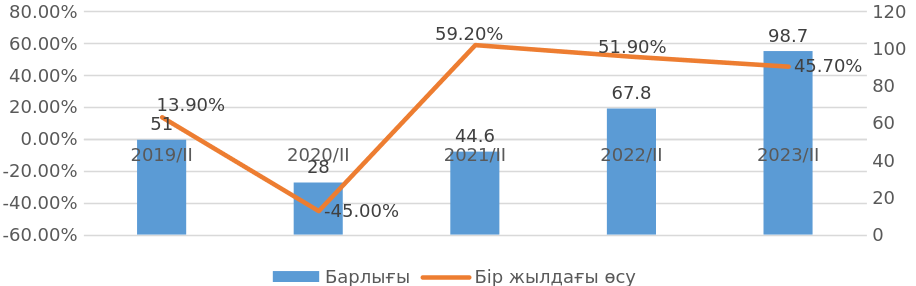
\includegraphics[width=0.6\textwidth]{media/ekon/image6.1}
	\caption*{1-сурет. Орналастыру орындарында көрсетілген қызметтер көлемі,
  млрд теңге}
  \caption*{Ескерту. Жасалған есептеулер негізінде авторлар құрастырған {[}7{]}}
\end{figure}



01.01.2022 ж. жағдай бойынша абсолютті өсім 13,365 млн теңгені құрады,
бұл пайыздық арақатынаста 17,69\% өсім ретінде көрсетіледі (2-сурет).



\begin{figure}[H]
	\centering
	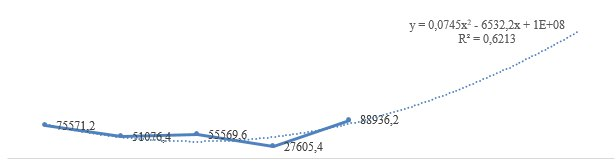
\includegraphics[width=0.6\textwidth]{media/ekon/image6.2}
	\caption*{2-сурет. Туроператорлар мен агенттіктердің экономикалық
  белсенділігі, млн теңге}
  \caption*{Ескерту. Жасалған есептеулер негізінде авторлар құрастырған {[}7{]}}
\end{figure}



Ұсынылған мәліметтерге сәйкес, жыл сайын ҚР-дағы Турфирмалар саны 10\% -
ға артады және келу және шығу туризмінің маңыздылығы, сондай-ақ ҚР
турфирмалары ұсынатын қызметтер сапасының артуы туралы куәландырады деп
болжауға болады (2-кесте).

{\bfseries 2-кесте-01.01.2022 ж. жағдай бойынша ҚР туристік қызметінің
көрсеткіштері}

\begin{longtable}[]{@{}
  >{\raggedright\arraybackslash}p{(\columnwidth - 12\tabcolsep) * \real{0.1521}}
  >{\raggedright\arraybackslash}p{(\columnwidth - 12\tabcolsep) * \real{0.0925}}
  >{\raggedright\arraybackslash}p{(\columnwidth - 12\tabcolsep) * \real{0.1182}}
  >{\raggedright\arraybackslash}p{(\columnwidth - 12\tabcolsep) * \real{0.1220}}
  >{\raggedright\arraybackslash}p{(\columnwidth - 12\tabcolsep) * \real{0.1456}}
  >{\raggedright\arraybackslash}p{(\columnwidth - 12\tabcolsep) * \real{0.1502}}
  >{\raggedright\arraybackslash}p{(\columnwidth - 12\tabcolsep) * \real{0.2195}}@{}}
\toprule\noalign{}
\multirow{3}{=}{\begin{minipage}[b]{\linewidth}\raggedright
Көрсеткіш
\end{minipage}} &
\multicolumn{4}{>{\raggedright\arraybackslash}p{(\columnwidth - 12\tabcolsep) * \real{0.4783} + 6\tabcolsep}}{%
\begin{minipage}[b]{\linewidth}\raggedright
Қызмет көрсетілгендер саны, мың адам
\end{minipage}} &
\multirow{3}{=}{\begin{minipage}[b]{\linewidth}\raggedright
Туристік қызметтен түсетін табыс, млн теңге
\end{minipage}} &
\multirow{3}{=}{\begin{minipage}[b]{\linewidth}\raggedright
Салықтар және бюджетке төленетін басқа да міндетті төлемдер, млн теңге
\end{minipage}} \\
& \multirow{2}{=}{\begin{minipage}[b]{\linewidth}\raggedright
Барлығы
\end{minipage}} &
\multicolumn{3}{>{\raggedright\arraybackslash}p{(\columnwidth - 12\tabcolsep) * \real{0.3858} + 4\tabcolsep}}{%
\begin{minipage}[b]{\linewidth}\raggedright
оның ішінде
\end{minipage}} \\
& & \begin{minipage}[b]{\linewidth}\raggedright
кіру
\end{minipage} & \begin{minipage}[b]{\linewidth}\raggedright
көшпелі
\end{minipage} & \begin{minipage}[b]{\linewidth}\raggedright
ішкі
\end{minipage} \\
\midrule\noalign{}
\endhead
\bottomrule\noalign{}
\endlastfoot
Олардың барлығы & 16598,6 & 4712,6 & 7412,3 & 4473,7 & 122004,3 &
40491,1 \\
Туристік ұйымдар & 486,5 & 39,7 & 274,6 & 172,2 & 21450,7 & 3277,9 \\
Орналастыру объектілері & 2458,9 & 594,2 & - & 1954,7 & 62082,2 &
33039,2 \\
Санаторий-курорттық мекемелермен & 218,9 & 65,7 & - & 153,2 & 13607,0 &
957,8 \\
Ерекше қорғалатын табиғи аумақтар & 537,9 & 162,0 & - & 375,1 & - & - \\
Мәдениет мекемелері & 3304,9 & 1486,3 & - & 1816,9 & 24863,6 & 3215,9 \\
\multicolumn{7}{@{}>{\raggedright\arraybackslash}p{(\columnwidth - 12\tabcolsep) * \real{1.0000} + 12\tabcolsep}@{}}{%
\emph{Ескерту. Жасалған есептеулер негізінде авторлар құрастырған
{[}7{]}}} \\
\end{longtable}

Қарастырылып отырған өсу жаһандық экономикалық және әлеуметтік
сын--қатерлерден, соның ішінде 2020 жылы салаға қатты әсер еткен
Covid-19 пандемиясынан туындаған құлдырау кезеңінен кейін туристік
индустрияның қалпына келуін және одан әрі дамуын көрсетеді. Қиындықтарға
қарамастан, туристік сектор тұрақтылық пен қалпына келтіру қабілетін
көрсетті, бұл туристік индустрияның ел экономикасы үшін маңыздылығын
растады {[}10{]}.

Туристік қызметтер саласындағы серпінді талдау көрсетілетін қызметтер
көлемінің тұрақты өсуінен және саланың экономикалық әлеуетін нығайтудан
көрінетін Қазақстандағы туристік саланы дамытудың оң үрдістерін растайды
(3-сурет).


\begin{figure}[H]
	\centering
	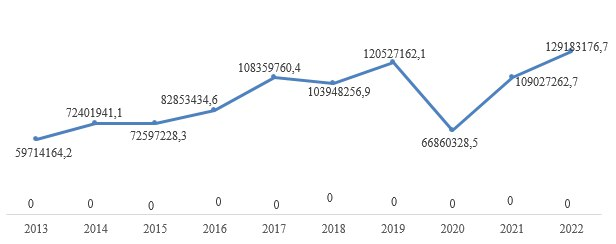
\includegraphics[width=0.6\textwidth]{media/ekon/image6.3}
	\caption*{3-сурет. ҚР орналастыру орындарымен көрсетілген қызметтер
  көлемі, мың теңге}
  \caption*{Ескерту. Жасалған есептеулер негізінде авторлар құрастырған {[}7{]}}
\end{figure}



Туризм индустриясын және ілеспе инфрақұрылымды дамыту Қазақстан
Республикасының туристік саласын дамытудың 2019-2025 жылдарға арналған
мемлекеттік бағдарламасын іске асыру шеңберінде негізгі бағыт болып
айқындалды. Туризм саласы туристік қызметтерге сұраныстың артуы,
туристік өнімдер ұсынысының кеңеюі, сондай-ақ саланы мемлекеттік қолдау
және ынталандыру сияқты әртүрлі факторларға байланысты тұрақты даму мен
кеңеюді көрсетеді.

Қазақстан Республикасында Туристік бизнесті дамыту мен ойын-сауық
саласындағы қызметтер көлемі арасындағы өзара байланыс туристік
сұранысты ынталандыру және туристерге қызмет көрсету сапасын жақсарту
үшін өте күшті және маңызды, сондықтан авторлар 2023-2025 жылдарға
арналған "ойын-сауық саласындағы қызметтер көлемі, млн. теңге"
көрсеткішінің болжамды мәндерін қарады.:

1. Ирвин критерийін қолдана отырып, қалыптан тыс бақылаулар үшін уақыт
қатарын тексеру (4-сурет)



\begin{figure}[H]
	\centering
	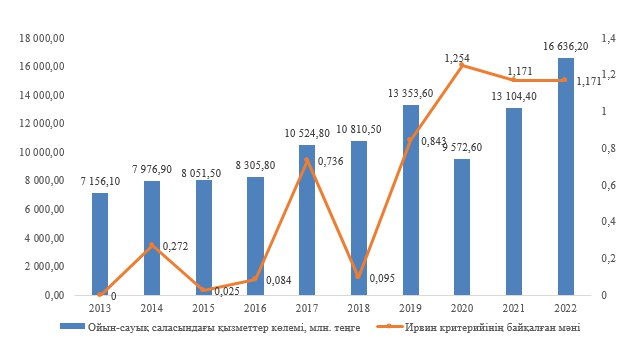
\includegraphics[width=0.6\textwidth]{media/ekon/image6.4}
	\caption*{4 -сурет Уақыт қатарында қалыптан тыс бақылаулардың болуын
  тексеру}
  \caption*{Ескерту. Жасалған есептеулер негізінде авторлар құрастырған {[}7{]}}
\end{figure}


Бұл жағдайда есептеу формулалары қолданылды:

- Ирвин критерийінің маңызды мәні

95\% жоғары сенімділікпен бастапқы уақыт қатарында аномальды бақылаулар
жоқ деп айтуға болады, өйткені Ирвин критерийі бойынша байқалған барлық
мәндер критикалық шектен аз болды. 2. Әрі қарай, қатардағы трендтің
болуын бағалау үшін "жоғары" және "төмен" сериялардың критерийлері
қарастырылды:

ықтималдығы бар есептелген мәнмен


ықтималдығы бар есептелген мәнмен

\textgreater{} 5).

3. Бастапқы деректерді жақындату үшін ең кіші квадраттар әдісін
қолдануды қарастырыңыз


4. Модельдің сапасын бағалау үшін екі тапсырма орындалды: - оның
сәйкестігін тексеру; - дәлдікті бағалау. Модельдің сәйкестігін тексеру
үшін бірқатар қалдықтарға талдау жасалды, бұл модельді қолдану арқылы
алынған болжамды мәндер мен нақты бақылаулар арасындағы айырмашылық.
Қалдықтардың маңызды сипаттамалары олардың математикалық күтуі,
кездейсоқтық және қалыпты үлестірімге сәйкестігі болып табылады.
Модельдің сәйкестігін тексеруге бағытталған қалдықтарды талдау
нәтижелері 4-кестеде келтірілген.

{\bfseries 4 - кесте. Болжамды анықтау үшін модельдің сәйкестігін тексеру}

% \begin{longtable}[]{@{}
%   >{\raggedright\arraybackslash}p{(\columnwidth - 4\tabcolsep) * \real{0.3638}}
%   >{\raggedright\arraybackslash}p{(\columnwidth - 4\tabcolsep) * \real{0.3486}}
%   >{\raggedright\arraybackslash}p{(\columnwidth - 4\tabcolsep) * \real{0.2877}}@{}}
% \toprule\noalign{}
% \multirow{2}{=}{\begin{minipage}[b]{\linewidth}\raggedright
% Тексерілетін қасиет
% \end{minipage}} &
% \multicolumn{2}{>{\raggedright\arraybackslash}p{(\columnwidth - 4\tabcolsep) * \real{0.6362} + 2\tabcolsep}@{}}{%
% \begin{minipage}[b]{\linewidth}\raggedright
% Қолданылатын статистика
% \end{minipage}} \\
% & \begin{minipage}[b]{\linewidth}\raggedright
% атауы, есептеу формуласы
% \end{minipage} & \begin{minipage}[b]{\linewidth}\raggedright
% алынған мән
% \end{minipage} \\
% \midrule\noalign{}
% \endhead
% \bottomrule\noalign{}
% \endlastfoot
% Кездейсоқтық & "Шыңдар" критерийі (бұрылыс
% \begin{figure}[H]
% 	\centering
% 	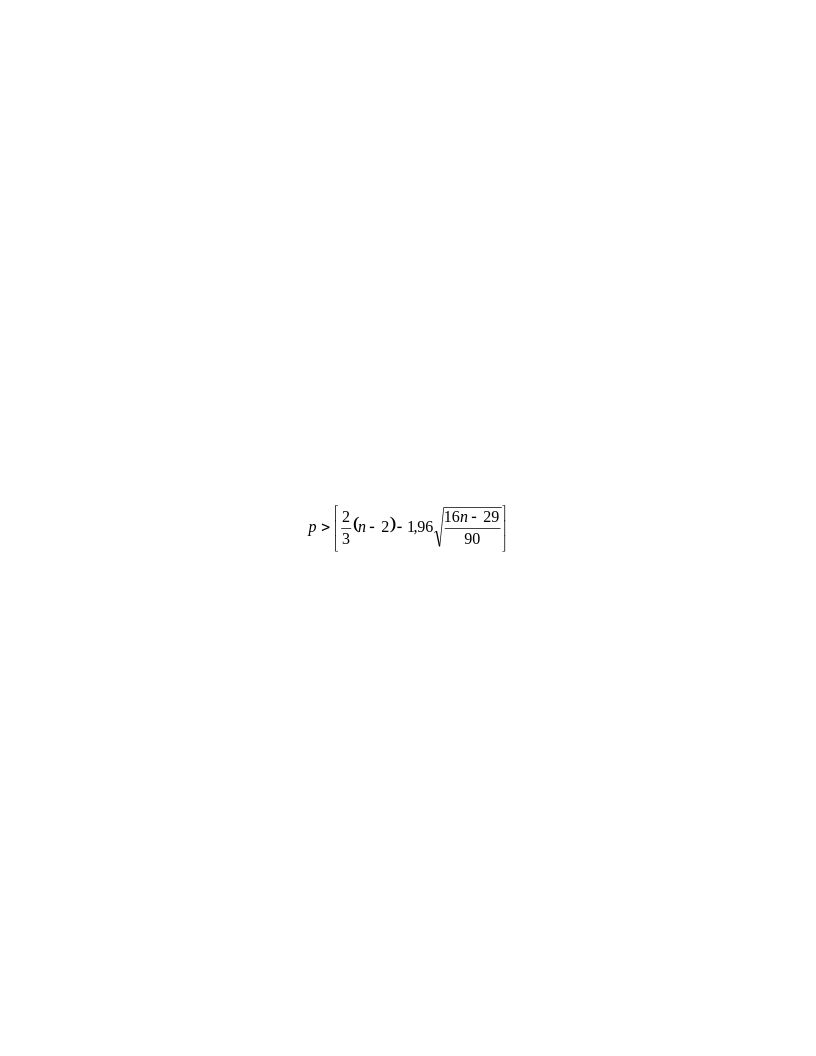
\includegraphics[width=0.8\textwidth]{media/ekon/image11}
% 	\caption*{}
% \end{figure}

% \textgreater{} 2 шекара кезінде 2 \\
% Қалыпты & RS-критерий

% \begin{figure}[H]
% 	\centering
% 	
\includegraphics[width=0.8\textwidth]{media/ekon/image12}
% 	\caption*{}
% \end{figure}

% кезінде 2,67-3,69 \\
% Қалдықтар қатарының деңгейлерін математикалық күтудің теңдігі нөлге тең
% & \emph{t}-статистика Стьюдента

% \begin{figure}[H]
% 	\centering
% 	
\includegraphics[width=0.8\textwidth]{media/ekon/image13}
% 	\caption*{}
% \end{figure}

% кезінде 2,31 \\
% \multicolumn{3}{@{}>{\raggedright\arraybackslash}p{(\columnwidth - 4\tabcolsep) * \real{1.0000} + 4\tabcolsep}@{}}{%
% \emph{*} Ескерту. Жүргізілген есептеулер негізінде авторлар
% құрастырған.} \\
% \end{longtable}

Жуықтаудың орташа салыстырмалы қателігі келесі мәнге


модельдің сәйкестігі мен дәлдігін көрсетеді.

5. Маңыздылық деңгейі кезінде 2025 жылға арналған" ойын - сауық
саласындағы қызметтер көлемі " көрсеткішінің нүктелік және аралық


оның келесі мәндері бар (сурет. 5).




\begin{figure}[H]
	\centering
	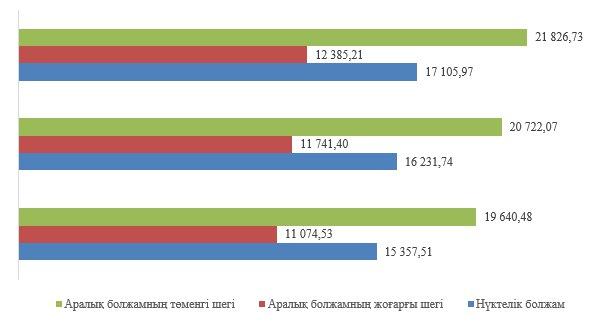
\includegraphics[width=0.6\textwidth]{media/ekon/image6.6}
	\caption*{5 - сурет. 01.01.2026 ж. жағдай бойынша "ойын-сауық саласындағы
  қызметтер көлемі" көрсеткішінің нүктелік және аралық болжамдары, млн
  теңг}
  \caption*{Ескерту. Жасалған есептеулер негізінде авторлар құрастырған {[}7{]}}
\end{figure}

Зерттеу туристік саланы дамытуға бағытталған басқару шешімдерін іске
асырудың тиімділігі елдің белгілі бір аймағындағы қонақ үй
индустриясының, инфрақұрылымның және қызмет көрсету саласының даму
деңгейіне тікелей байланысты деген қорытынды жасауға мүмкіндік береді.
Қорытындылар. Қазақстан Республикасының туристік саласын дамыту оң
серпінді көрсетіп отыр, алайда ағымдағы сын-қатерлерді еңсеру және оның
ұлттық экономикаға қосқан үлесін ұлғайту үшін одан әрі стратегиялық
тәсілді талап етеді.

{\bfseries Қорытынды.} Зерттеу көрсеткендей, 2022 жылы туристер саны 9
миллионнан асты, бұл 2021 жылмен салыстырғанда 20\% - ға өсті.

Туристік қызметтен түсетін табыс 2021 жылғы 88,9 млрд теңгеден 2023
жылдың басындағы 98,7 млрд теңгеге дейін ұлғайды. Деректер тиімді
пайдаланылуы қажет саланың айтарлықтай әлеуетін көрсетеді. Талдау
көрсеткендей, инновациялық технологияларды енгізу және инфрақұрылымды
жаңарту туристік саланың өсуіне ықпал етеді. Мысалы, цифрлық
технологияларды енгізу туристік қызметтердің сапасын жақсартады, ал
инфрақұрылымға стратегиялық инвестициялар туристерді көбірек тартуға
мүмкіндік береді. 2022 жылы туристер санының 20\% - ға ұлғаюы, туризмнен
түсетін табыстың 98,7 млрд теңгеге дейін өсуі, сондай-ақ қонақ үй
секторының 70\% жүктемемен кеңеюі ұсынылған тәсілдердің тиімділігін
растайды. Дегенмен, тұрақтылыққа қол жеткізу үшін ағымдағы кедергілерді,
соның ішінде сапалы қонақүйлердің тапшылығын және экскурсиялық
инфрақұрылымның жеткіліксіз дамуын жою қажет. Демек, гипотеза расталады:
инновациялық тәсілдер мен стратегиялық инвестициялар экономикалық
әлеуетті нығайта отырып, туризмнің дамуына ықпал етеді. Туризмнің
әлемдік индустрияға қосқан үлесі шектеулі болып қалады, бұл жаһандық
туристік ағынның 1\% - дан азын құрайды.

Өсудің негізгі кедергілері инфрақұрылымдық шектеулер, соның ішінде
сапалы қонақ үй қызметтерінің тапшылығы және белсенді және мәдени туризм
үшін объектілердің жеткіліксіз дамуы болып табылады. Қазақстанда 2023
жылдың басында 2851 қонақ үй болды, оның 228-і халықаралық стандарттарға
сәйкес келеді, орташа жүктемесі 70 \%. Көрсеткіштер саланың тұрақты
өсуін қамтамасыз ету үшін инфрақұрылымды жаңғырту және кеңейту
қажеттігін көрсетеді.

Мемлекеттік қолдау, атап айтқанда туризмді дамыту бағдарламаларын іске
асыру және кластерлік тәсілді енгізу бәсекеге қабілеттілікті жақсартуда
басты рөл атқарады. Бұдан басқа, цифрлық технологияларды пайдалану
көрсетілетін қызметтердің сапасын арттыруға және тартымды туристік бағыт
ретінде Қазақстанның халықаралық имиджін нығайтуға мүмкіндік береді.
Ұлттық саябақтарды қоса алғанда, 200-ден астам қорғалатын табиғи
аумақтарға негізделген экологиялық және мәдени туризм ұтымды пайдалануды
және одан әрі ілгерілеуді қажет ететін маңызды ресурс болып табылады.
Туристік индустрияның ұзақ мерзімді табысы үшін кедергілерді жоюға,
соның ішінде көлікке қолжетімділікті жақсартуға, әкімшілік
процедураларды жеңілдетуге және инновациялық шешімдерді енгізуге назар
аудару қажет.

Туризмді халықаралық ілгерілету үшін инфрақұрылымға стратегиялық
инвестициялау және маркетингтік науқандарды дамыту сектордың тұрақты
дамуын қамтамасыз етеді. Жүргізілген талдау нәтижесінде туризм
экономикалық өсудің маңызды драйвері болып табылатыны расталды. Оның
әлеуетін барынша ашу үшін қызмет көрсету сапасын арттыруға,
инфрақұрылымды дамытуға және кәсіпкерлік белсенділікті арттыруға
бағытталған стратегиялық бастамаларды жалғастыру қажет. Ресурстарды
тиімді басқару және ағымдағы кемшіліктерді жою Қазақстанның жаһандық
туристік картадағы орнықты өсуі мен ұстанымын нығайту үшін жағдай
жасайды.

{\bfseries Литература}

\begin{enumerate}
\def\labelenumi{\arabic{enumi}.}
\item
  Solvoll S., Bulanova J., Alsos G.A. Tourism Entrepreneurship -- Review
  and Future Directions // Scandinavian Journal of Hospitality and
  Tourism.- 2015.- Vol.15. - P.120-137
\end{enumerate}

DOI
\href{http://dx.doi.org/10.1080/15022250.2015.1065592}{10.1080/15022250.2015.1065592}

\begin{enumerate}
\def\labelenumi{\arabic{enumi}.}
\setcounter{enumi}{1}
\item
  Yanyun Z, Bingjie L The evolution and new trends of
  China' s tourism industry // National Accounting
  Review. -2020.
  -\href{https://www.aimspress.com/nar/article/archives}{Vol.2}.(4). -
  P. 337-353. DOI
  \href{https://doi.org/10.3934/NAR.2020020}{10.3934/NAR.2020020}
\item
  Tian Jie, Tan Qiuyun, Jin JingyuCan Digital Finance Improve
  Misallocation of Resourses/~J.~Tian, K.~Tang, J.~Jin //~Col. S. Fin.
  Econ.
  -\href{https://cjlc.zufe.edu.cn/EN/article/showTenYearVolumnDetail.do?nian=2021}{2021}.
  -\href{https://cjlc.zufe.edu.cn/EN/article/showTenYearVolumnDetail.do?nian=2021}{Vol.
  37}\href{file:///C:/Users/admin/Desktop/Вестник\%20КазУТБ/4\%202024/(4)}{(4)}.
  - P.49-60.
\end{enumerate}

URL: \url{https://cjlc.zufe.edu.cn/EN/Y2021/V37/I4/49}

\begin{enumerate}
\def\labelenumi{\arabic{enumi}.}
\setcounter{enumi}{3}
\item
  Арынова Ж.З., Арынова Ж.З., Нурмаганбетова А.Ж.~, Искакова А.Т.,
  Тебаев Ж.Ж.~ Условия повышения конкурентоспособности субъектов
  предпринимательства индустрии туризма Казахстана // Вестн. Казах.
  ун-та экон., финансов и междунар. торговли. -2022. -№ 2(47). - С.
  298-304. DOI10.52260/2304-7216.2022.2(47).41
\item
  Асетова А.А. Особенности конкурентоспособности туристического бизнеса
  в Казахстане: обзор литературы // Инновации. Наука. Образование.
  -2021. -№ 48. -С. 357-367.
\end{enumerate}

https://innovjourn.ru/nomer/48-nomer/

\begin{enumerate}
\def\labelenumi{\arabic{enumi}.}
\setcounter{enumi}{5}
\item
  Тлеубердинова А.Т., ШаекинаЖ.М., СалауатоваД.М., Stephen Pratt.
  Факторный анализ развития туристского предпринимательства в
  Казахстане. // Экономика: стратегия и практика. - 2020. -№ 1 (15). -С.
  79-89. DOI 10.51176/JESP/issue\_1\_T6
\item
  Вечкинзова Е.А. Сравнительный анализ развития региональной
  индустриально-инновационной инфраструктуры России и Казахстана //
  Экономика Центральной Азии. - 2019. -Т. 3,-№ 1. -C. 19-34. DOI
  10.18334/asia.3.1.40757
\item
  Рахметова Д.А., Д.А.~Рахметова., А.А.~Нургалиева., С.~Дырка.,
  Г.Ы.~Бекенова., Г.А.~Оспанова. Направления развития туристской
  предпринимательской деятельности в Республике Казахстан. //~Bulletin
  the National academy of sciences of the Republic of Kazakhstan.
  -2023.-№ 5.~-С. 525-541. DOI 10.32014/2023.2518-1467.607
\item
  Аубакирова Г.М. Новые подходы к построению модели экономического роста
  Казахстана//Экономические отношения.- 2019.-№ 1.-C.123-124. DOI
  10.18334/eo.9.1.39729
\end{enumerate}

10.Бюро национальной статистики Агентства по стратегическому
планированию и реформам РК. Статистика туризма. URL:
\url{https://stat.gov.kz/official/industry/22/statistic/7}

{\bfseries References}

1. Solvoll S., Bulanova J., Alsos G.A. Tourism Entrepreneurship --
Review and Future Directions // Scandinavian Journal of Hospitality and
Tourism.- 2015.- Vol.15. - P.120-137

DOI
\href{http://dx.doi.org/10.1080/15022250.2015.1065592}{10.1080/15022250.2015.1065592}

2. Yanyun Z, Bingjie L The evolution and new trends of
China' s tourism industry // National Accounting Review.
-2020.
-\href{https://www.aimspress.com/nar/article/archives}{Vol.2}.(4). - P.
337-353. DOI
\href{https://doi.org/10.3934/NAR.2020020}{10.3934/NAR.2020020}

3. Tian Jie, Tan Qiuyun, Jin JingyuCan Digital Finance Improve
Misallocation of Resourses/~J.~Tian, K.~Tang, J.~Jin //~Col. S. Fin.
Econ.
-\href{https://cjlc.zufe.edu.cn/EN/article/showTenYearVolumnDetail.do?nian=2021}{2021}.
-\href{https://cjlc.zufe.edu.cn/EN/article/showTenYearVolumnDetail.do?nian=2021}{Vol.
37}\href{file:///C:/Users/admin/Desktop/Вестник\%20КазУТБ/4\%202024/(4)}{(4)}.
- P.49-60.

URL: \url{https://cjlc.zufe.edu.cn/EN/Y2021/V37/I4/49}

4. Arynova Zh.Z., Arynova Zh.Z., Nurmaganbetova A.Zh. , Iskakova A.T.,
Tebaev Zh.Zh. Uslovija povyshenija konkurentosposobnosti sub\#ektov
predprinimatel' stva industrii turizma Kazahstana //
Vestn. Kazah. un-ta jekon., finansov i mezhdunar. torgovli. -2022. -№
2(47). - S. 298-304. DOI10.52260/2304-7216.2022.2(47).41 {[}in
Russian{]}

5.Asetova A.A. Osobennosti konkurentosposobnosti turisticheskogo biznesa
v Kazahstane: obzor literatury // Innovacii. Nauka. Obrazovanie. -2021.
-№ 48. -S. 357-367.

https://innovjourn.ru/nomer/48-nomer/.{[}in Russian{]}

6.Tleuberdinova A.T., ShaekinaZh.M., SalauatovaD.M., Stephen Pratt.
Faktornyj analiz razvitija turistskogo
predprinimatel' stva v Kazahstane. // Jekonomika:
strategija i praktika. - 2020. -№ 1 (15). -S. 79-89. DOI
10.51176/JESP/issue\_1\_T6. {[}in Russian{]}

7.Vechkinzova E.A. Sravnitel' nyj analiz razvitija
regional' noj industrial' no-innovacionnoj
infrastruktury Rossii i Kazahstana // Jekonomika
Central' noj Azii. - 2019. -T. 3,-№ 1. -C. 19-34. DOI
10.18334/asia.3.1.40757. {[}in Russian{]}

8.Rahmetova D.A., D.A. Rahmetova., A.A. Nurgalieva., S. Dyrka., G.Y.
Bekenova., G.A. Ospanova. Napravlenija razvitija turistskoj
predprinimatel' skoj dejatel' nosti v
Respublike Kazahstan. // Bulletin the National academy of sciences of
the Republic of Kazakhstan. -2023.-№ 5. -S. 525-541. DOI
10.32014/2023.2518-1467.607. {[}in Russian{]}

9.Aubakirova G.M. Novye podhody k postroeniju modeli jekonomicheskogo
rosta Kazahstana//Jekonomicheskie otnoshenija.- 2019.-№ 1.-C.123-124.
DOI 10.18334/eo.9.1.39729. {[}in Russian{]}

10.Bjuro nacional' noj statistiki Agentstva po
strategicheskomu planirovaniju i reformam RK. Statistika turizma. URL:
\url{https://stat.gov.kz/official/industry/22/statistic/7}. {[}in
Russian{]}

\emph{{\bfseries Авторлар туралы мәліметтер}}

А.Сабыржан\textsuperscript{.} - э.ғ.к., доцент м.а., Е.А.Бөкетов
атындағы Қарағанды университеті, Қарағанды, Қазақстан, e-mail:
Alisher-aliev-79@mail.ru;

Г.Қ. Абдраманова - э.ғ.к., доцент м.а., Л.Н. Гумилев атындағы Еуразия
ұлттық университеті, Астана, Қазақстан, e-mail:
\href{mailto:agk2009@mail.ru}{\nolinkurl{agk2009@mail.ru}};

А.Т.Тлеубаева - PhD, доцент м.а., Л.Н. Гумилев атындағы Еуразия ұлттық
университеті, Астана, Қазақстан, e-mail: aitolkyn.t@mail.ru,
tleubayeva\_at@enu.kz;

М.С.Сиеубаева - Ғылым магистрі, аға оқытушы, Л.Н.Гумилёв атындағы
Еуразия ұлттық университеті, Астана, Қазақстан, e-mail:
sieubayeva\_ms@enu.kz.

\emph{{\bfseries Information about the authors}}

A.Sabyrzhan - Candidate of Economic Sciences, Acting Associate
Professor{\bfseries ,} Karaganda Buketov University, Karaganda, Kazakhstan,
e-mail: Alisher-aliev-79@mail.ru;

G. Abdramanova {\bfseries -} Candidate of Economic Sciences, Acting
Associate Professor{\bfseries ,} L.N. Gumilyov Eurasian National
University, Astana, Kazakhstan, e-mail:
\href{mailto:agk2009@mail.ru}{\nolinkurl{agk2009@mail.ru}};

A. Tleubayeva - PhD, acting Associate Professor, L.N. Gumilyov Eurasian
National University, Astana, Kazakhstan, e-mail: aitolkyn.t@mail.ru,
\href{mailto:tleubayeva_at@enu.kz}{\nolinkurl{tleubayeva\_at@enu.kz}};

M. Siyeubayeva - Master of Science, senior lecturer, L.N. Gumilyov
Eurasian National University, Astana, Kazakhstan, e-mail:
\href{mailto:sieubayeva_ms@enu.kz}{\nolinkurl{sieubayeva\_ms@enu.kz}}.